% \VignetteIndexEntry{grim - Graphical Interaction Models}
% \VignetteDepends{gRbase}
% \VignetteKeyword{Graphical Models}
% \VignetteKeyword{Hierarchical log-linear models}
% \VignetteKeyword{Graphical Gaussian models}

\documentclass[12pt]{article}

%% For Danish letters.
\usepackage[T1]{fontenc}
\usepackage[latin1]{inputenc}
\usepackage{GMIR}
\usepackage{Sweave,amsmath,amsfonts,bm,color}
%%\usepackage[authoryear,round]{natbib}
\bibliographystyle{plainnat}
\usepackage{a4wide}
%%\usepackage[inline,nomargin,draft]{fixme}
%%\usepackage{natbib}
\usepackage{boxedminipage}
\usepackage{shortvrb}
\MakeShortVerb|




\title{On the usage of the \pkg{gRim} package}
\author{S{\o}ren H{\o}jsgaard}
\date{\pkg{gRim} version 0.2.2 as of 2020-06-14}


\begin{document}
\Sconcordance{concordance:grim.tex:grim.Rnw:%
1 23 1 1 6 46 1 1 8 3 1 1 8 28 1 1 3 8 0 1 1 6 0 1 1 7 0 1 2 14 1 1 3 1 0 1 %
1 13 0 1 2 8 1 1 3 1 0 3 1 9 0 1 2 16 1 1 3 6 0 1 1 8 0 1 2 2 1 1 3 12 0 1 %
2 27 1 1 4 2 0 1 1 7 0 1 2 1 4 2 0 1 1 6 0 1 2 10 1 1 3 5 0 1 2 10 1 1 3 1 %
0 3 1 9 0 1 2 2 1 1 3 5 0 1 2 3 1 1 3 1 0 2 1 9 0 1 2 2 1 1 3 5 0 1 2 13 1 %
1 3 1 0 1 1 6 0 1 2 2 1 1 3 1 0 1 1 6 0 1 2 2 1 1 3 1 0 1 1 6 0 1 2 2 1 1 3 %
1 0 1 1 6 0 1 2 2 1 1 3 1 0 1 1 7 0 1 2 2 1 1 3 1 0 1 1 6 0 1 2 2 1 1 3 1 0 %
1 1 6 0 1 2 17 1 1 3 14 0 1 2 29 1 1 3 11 0 1 2 28 1 1 3 14 0 1 2 7 1 1 4 %
11 0 1 2 1 5 16 1 1 3 8 0 1 1 8 0 1 2 15 1 1 3 9 0 1 2 22 1 1 3 12 0 1 2 9 %
1 1 3 9 0 1 2 4 1 1 3 8 0 1 1 8 0 1 2 10 1 1 4 13 0 1 2 18 1 1 3 1 0 1 1 11 %
0 1 1 4 0 1 2 11 1 1 3 1 0 1 1 8 0 1 1 4 0 1 2 60 1 1 3 1 0 2 1 9 0 1 1 11 %
0 1 2 7 1 1 3 10 0 1 2 202 1 1 3 7 0 1 2 50 1 1 4 2 0 1 1 6 0 1 2 4 1 1 3 9 %
0 1 2 1 3 7 0 1 2 2 1 1 3 7 0 1 2 5 1 1 2 10 0 1 2 222 1}


\setkeys{Gin}{width=0.5\textwidth,height=2in} %sæt figurstørrelse i Sweave
\renewenvironment{Schunk}{\linespread{.85}\scriptsize}{}

\definecolor{myGray}{rgb}{0.95,0.95,0.95}
\makeatletter
\renewenvironment{Schunk}{
  \begin{lrbox}{\@tempboxa}
    \begin{boxedminipage}
      {\columnwidth}\small}
    {\end{boxedminipage}
  \end{lrbox}%
  \colorbox{myGray}{\usebox{\@tempboxa}}
}
\makeatother


\maketitle
\tableofcontents

\parindent0pt\parskip5pt


\def\dmod{\texttt{dmod}}
\def\cmod{\texttt{cmod}}
\def\mmod{\texttt{mmod}}

\def\imodo{\texttt{iModel}}
\def\dmodo{\texttt{dModel}}
\def\cmodo{\texttt{cModel}}
\def\mmodo{\texttt{mModel}}


\def\rformula#1{\texttt{\~{ }#1}}
\def\carcass{\texttt{carcass}}
\def\reinis{\texttt{reinis}}
\def\mildew{\texttt{mildew}}




\section{Introduction}



The \grim\ package is an \R\ package for \emph{gRaphical interaction
  models} (hence the name).  \grim\ implements 1) graphical
log--linear models for discrete data, that is for contingency tables
and 2) Gaussian graphical models for continuous data (multivariate
normal data) and 3) mixed homogeneous interaction models for mixed
data (data consisiting of both discrete and continuous variables).

The package is at an early stage of development and so is this
document.


\section{Introductory examples}
\label{sec:introex}

The main functions for creating models of the various types are:

\begin{itemize}
\item Discrete data: The \comi{dmod()} function creates a hierarchical
  log--linear model.
\item Continuous data: The \comi{cmod()} function creates a Gaussian
  graphical model.
\item Mixed data: The \comi{mmod()} function creates a mixed
  interaction model.
\end{itemize}

The arguments to the model functions are:

\begin{Schunk}
\begin{Sinput}
> args(dmod)
\end{Sinput}
\begin{Soutput}
function (formula, data, marginal = NULL, interactions = NULL, 
    fit = TRUE, details = 0, ...) 
NULL
\end{Soutput}
\begin{Sinput}
> args(cmod)
\end{Sinput}
\begin{Soutput}
function (formula, data, marginal = NULL, fit = TRUE, details = 0) 
NULL
\end{Soutput}
\begin{Sinput}
> args(mmod)
\end{Sinput}
\begin{Soutput}
function (formula, data, marginal = NULL, fit = TRUE, details = 0) 
NULL
\end{Soutput}
\end{Schunk}


The model objects created by these functions are of the respective
classes \dmodo, \cmodo\ and \mmodo. All models are also of the class
\imodo.  We focus the presentation on models for discrete data, but
most of the topics we discuss apply to all types of models.



\subsection{A Discrete Model}
\label{sec:xxx}


The \comi{reinis} data from \grbase\ is a $2^6$ contingency table.

\begin{Schunk}
\begin{Sinput}
> data(reinis)
> str(reinis)
\end{Sinput}
\begin{Soutput}
 'table' num [1:2, 1:2, 1:2, 1:2, 1:2, 1:2] 44 40 112 67 129 145 12 23 35 12 ...
 - attr(*, "dimnames")=List of 6
  ..$ smoke  : chr [1:2] "y" "n"
  ..$ mental : chr [1:2] "y" "n"
  ..$ phys   : chr [1:2] "y" "n"
  ..$ systol : chr [1:2] "y" "n"
  ..$ protein: chr [1:2] "y" "n"
  ..$ family : chr [1:2] "y" "n"
\end{Soutput}
\end{Schunk}

Models are specified as generating classes. A generating class can be
a list or a right--hand--sided formula. In addition, various model
specification shortcuts are available.  Some of these are described in
Section~\ref{sec:shortcut}.

The following two
specifications of a log--linear model are equivalent:

\begin{Schunk}
\begin{Sinput}
> data(reinis)
> dm1<-dmod(list(c("smoke","systol"),c("smoke","mental","phys")), data=reinis)
> dm1<-dmod(~smoke:systol + smoke:mental:phys, data=reinis)
> dm1
\end{Sinput}
\begin{Soutput}
Model: A dModel with 4 variables
 -2logL    :        9391.38 mdim :    9 aic :      9409.38 
 ideviance :         730.47 idf  :    5 bic :      9459.05 
 deviance  :           3.80 df   :    6 
\end{Soutput}
\end{Schunk}

The output reads as follows: |-2logL| is minus twice the maximized
log--likelihood and |mdim| is the number of parameters in the model
(no adjustments have been made for sparsity of data).
The |ideviance| and |idf| gives the deviance and degrees of
freedom between the model and the independence model for the same
variables and |deviance| and |df| is the deviance and degrees of
freedom between the model and the saturated model for the same
variables.

Section~\ref{sec:intomodel} describes model objects in more
detail. Here we just notice that the generating class of the model is
contained in the slot \code{glist}:

Notice that the generating class does not appear directly. However the
generating class can be retrieved using \comi{formula()} and \comi{terms()}:

\begin{Schunk}
\begin{Sinput}
> formula(dm1)
\end{Sinput}
\begin{Soutput}
~smoke * mental * phys + smoke * systol
\end{Soutput}
\begin{Sinput}
> str(terms(dm1))
\end{Sinput}
\begin{Soutput}
List of 2
 $ : chr [1:3] "smoke" "mental" "phys"
 $ : chr [1:2] "smoke" "systol"
\end{Soutput}
\end{Schunk}

A summary of a model is provided by the \comi{summary()} function:

\begin{Schunk}
\begin{Sinput}
> summary(dm1)
\end{Sinput}
\begin{Soutput}
          Length Class  Mode     
modelinfo 3      -none- list     
varNames  4      -none- character
datainfo  1      -none- list     
fitinfo   9      -none- list     
isFitted  1      -none- logical  
\end{Soutput}
\end{Schunk}

\footnote{The summary() method leaves a bit to be desired...}



\subsection{Model specification shortcuts}
\label{sec:shortcut}

Below we illustrate various other ways of specifying log--linear
models.

\begin{itemize}
\item A saturated model can be specified using \verb|~.^.| whereas
\verb|~.^2| specifies the model with all--two--factor
interactions. Using \verb|~.^1| specifies the independence model.

\item If we want, say, at most two--factor interactions in the
model we can use the |interactions| argument.

\item Attention can be restricted to a subset of the variables
using the |marginal| argument.

\item Variable names can be abbreviated.

\end{itemize}

The following models illustrate these abbreviations:

\begin{Schunk}
\begin{Sinput}
> dm2 <- dmod(~.^2, margin=c("smo","men","phy","sys"),
+             data=reinis)
> formula(dm2)
\end{Sinput}
\begin{Soutput}
~smoke * mental + smoke * phys + mental * phys + smoke * systol + 
    mental * systol + phys * systol
\end{Soutput}
\end{Schunk}

\begin{Schunk}
\begin{Sinput}
> dm3 <- dmod(list(c("smoke", "systol"), c("smoke", "mental", "phys")),
+             data=reinis, interactions=2)
> formula(dm3)
\end{Sinput}
\begin{Soutput}
~smoke * mental + smoke * phys + mental * phys + smoke * systol
\end{Soutput}
\end{Schunk}

\subsection{Plotting models}
\label{sec:xxx}

There are two methods for plotting the dependence graph of a model:
Using \comi{iplot()} and \comi{plot()}. The convention for both
methods is that discrete variables are drawn as grey dots and
continuous variables as white dots.  1) \comi{iplot()} creates an
\code{igraph} object and plots this. 2) 2) \comi{plot()} creates a
\code{graphNEL} object and plots this.

\begin{Schunk}
\begin{Sinput}
> iplot(dm1)
\end{Sinput}
\end{Schunk}
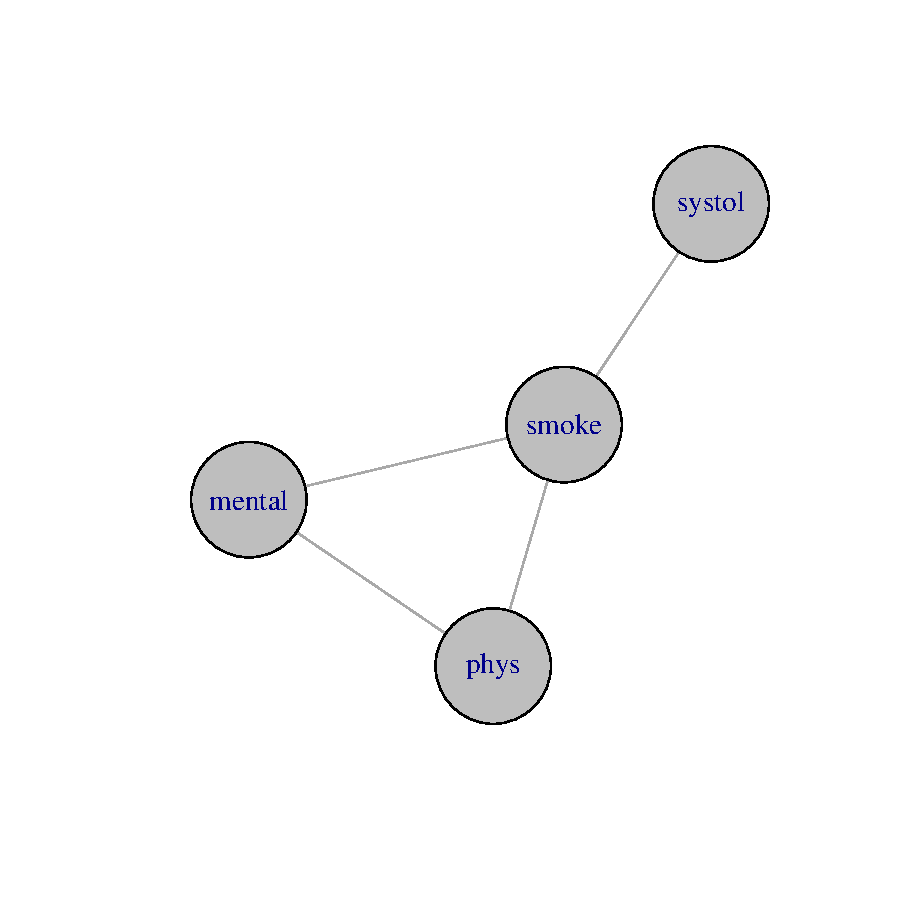
\includegraphics{figures/GRIM-011}





\subsection{A Continuous Model}
\label{sec:xxx}

For Gaussian models there are at most second order interactions. Hence
we may specify the saturated model in different ways:

\begin{Schunk}
\begin{Sinput}
> data(carcass)
> cm1 <- cmod(~Fat11:Fat12:Fat13, data=carcass)
> cm1 <- cmod(~Fat11:Fat12 + Fat12:Fat13 + Fat11:Fat13, data=carcass)
> cm1
\end{Sinput}
\begin{Soutput}
Model: A cModel with 3 variables
 -2logL    :        4329.16 mdim :    6 aic :      4341.16 
 ideviance :         886.10 idf  :    3 bic :      4364.20 
 deviance  :           0.00 df   :    0 
\end{Soutput}
\end{Schunk}

\footnote{Harmonize cmod() output with that of dmod()}

\begin{Schunk}
\begin{Sinput}
> iplot(cm1)
\end{Sinput}
\end{Schunk}
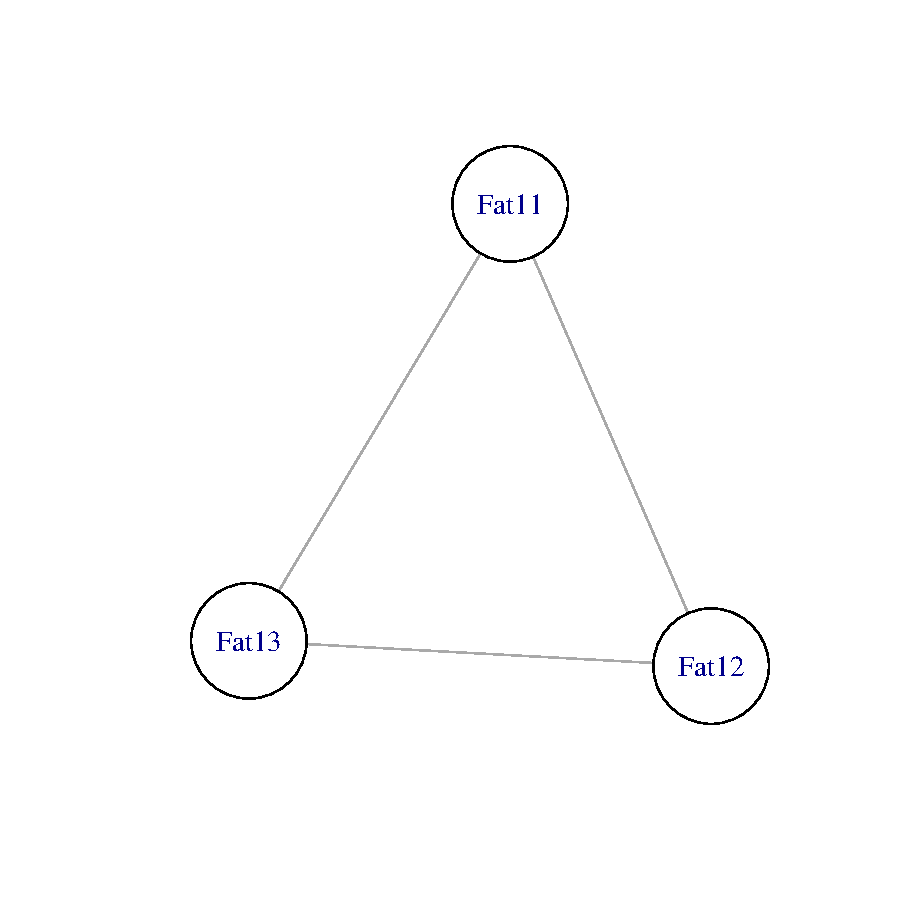
\includegraphics{figures/GRIM-013}


\subsection{A Mixed Model}

\begin{Schunk}
\begin{Sinput}
> data(milkcomp1)
> mm1 <- mmod(~.^., data=milkcomp1)
> mm1
\end{Sinput}
\begin{Soutput}
Model: A mModel with 5 variables
 -2logL    :         475.92 mdim :   44 aic :       563.92 
 ideviance :         101.57 idf  :   31 bic :       652.24 
 deviance  :           0.00 df   :    0 
\end{Soutput}
\end{Schunk}

\footnote{Harmonize mmod() output with that of dmod()}

\begin{Schunk}
\begin{Sinput}
> iplot(mm1)
\end{Sinput}
\end{Schunk}
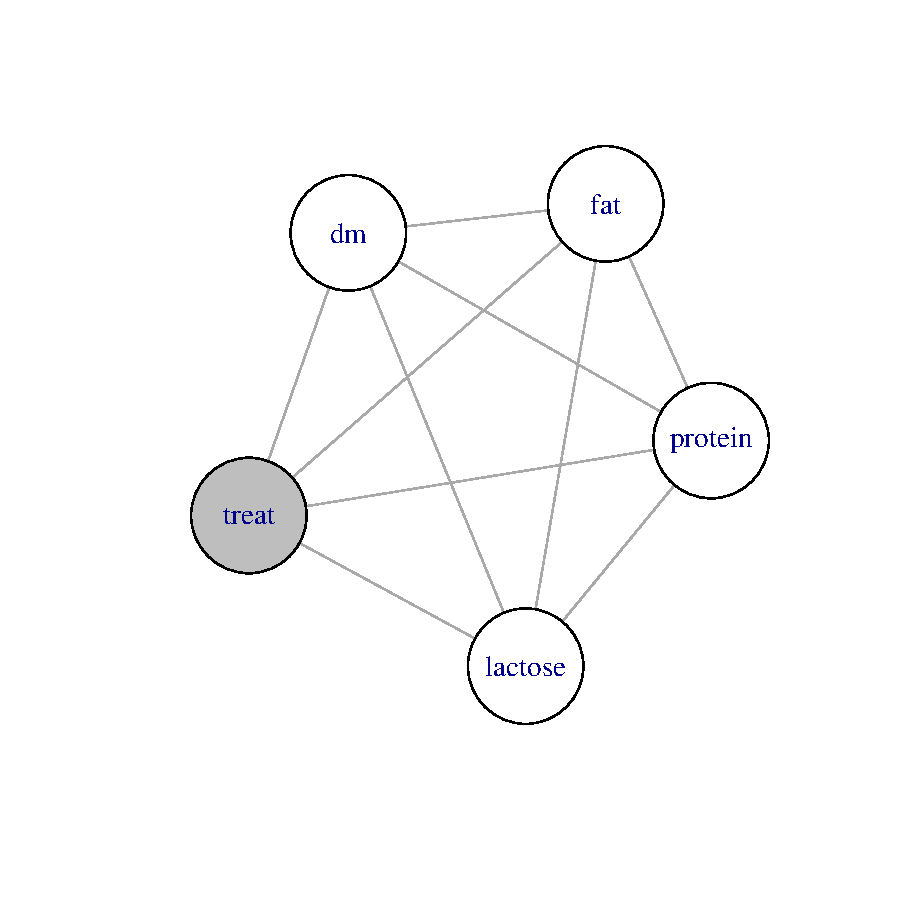
\includegraphics{figures/GRIM-015}




\section{Model editing - \code{update()}}

The \comi{update()} function enables \dmodo\ objects to be modified by the addition
or deletion of interaction terms or edges, using the arguments \code{aterm}, \code{dterm},
\code{aedge} or \code{dedge}. Some examples follow:


\begin{itemize}
\item Set a marginal saturated model:

\begin{Schunk}
\begin{Sinput}
> ms <- dmod(~.^., marginal=c("phys","mental","systol","family"), data=reinis)
> formula(ms)
\end{Sinput}
\begin{Soutput}
~phys * mental * systol * family
\end{Soutput}
\end{Schunk}

\item Delete one edge:

\begin{Schunk}
\begin{Sinput}
> ms1 <- update(ms, list(dedge=~phys:mental))
> formula(ms1)
\end{Sinput}
\begin{Soutput}
~phys * systol * family + mental * systol * family
\end{Soutput}
\end{Schunk}

\item Delete two edges:

\begin{Schunk}
\begin{Sinput}
> ms2<- update(ms, list(dedge=~phys:mental+systol:family))
> formula(ms2)
\end{Sinput}
\begin{Soutput}
~phys * systol + phys * family + mental * systol + mental * family
\end{Soutput}
\end{Schunk}

\item Delete all edges in a set:

\begin{Schunk}
\begin{Sinput}
> ms3 <- update(ms, list(dedge=~phys:mental:systol))
> formula(ms3)
\end{Sinput}
\begin{Soutput}
~phys * family + mental * family + systol * family
\end{Soutput}
\end{Schunk}

\item Delete an interaction term

\begin{Schunk}
\begin{Sinput}
> ms4 <- update(ms, list(dterm=~phys:mental:systol) )
> formula(ms4)
\end{Sinput}
\begin{Soutput}
~phys * mental * family + phys * systol * family + mental * systol * 
    family
\end{Soutput}
\end{Schunk}

\item Add three interaction terms:

\begin{Schunk}
\begin{Sinput}
> ms5 <- update(ms, list(aterm=~phys:mental+phys:systol+mental:systol) )
> formula(ms5)
\end{Sinput}
\begin{Soutput}
~phys * mental * systol * family
\end{Soutput}
\end{Schunk}

\item Add two edges:

\begin{Schunk}
\begin{Sinput}
> ms6 <- update(ms, list(aedge=~phys:mental+systol:family))
> formula(ms6)
\end{Sinput}
\begin{Soutput}
~phys * mental * systol * family
\end{Soutput}
\end{Schunk}
\end{itemize}

A brief explanation of these operations may be helpful. To obtain a hierarchical model when
we delete a term from a model, we must delete any higher-order relatives to the term.
Similarly, when we add an interaction term we must also add all lower-order relatives that
were not already present. Deletion of an edge is equivalent to deleting the corresponding
two-factor term. Let $m-e$ be the result of deleting edge $e$ from a model $m$. Then the
result of adding $e$ is defined as the maximal model $m^*$ for which $m^*-e=m$.



\section{Testing for conditional independence}
\label{sec:citest}

Tests of general conditional independence hypotheses of the form $u
\cip v \cd W$ can be performed using the \comics{ciTest()}{\grim}
function.

\begin{Schunk}
\begin{Sinput}
> cit <- ciTest(reinis, set=c("systol","smoke","family","phys"))
\end{Sinput}
\begin{Soutput}
Testing systol _|_ smoke | family phys 
Statistic (DEV):   13.045 df: 4 p-value: 0.0111 method: CHISQ
Slice information:
  statistic  p.value df family phys
1  4.734420 0.029565  1      y    y
2  0.003456 0.953121  1      n    y
3  7.314160 0.006841  1      y    n
4  0.993337 0.318928  1      n    n
\end{Soutput}
\end{Schunk}

The general syntax of the \code{set} argument is of the form $(u,v,W)$
where $u$ and $v$ are variables and $W$ is a set of variables.
The \code{set} argument can also be given as a right--hand sided formula.

% Notice that in this case the results are identical to those of
% \comics{testdelete()}{\grim}, since we have specified the correct
% conditioning set. If we had conditioned on more variables

% @
% <<print=T>>=
% cit2 <- CItest(mildew, set=c("locc","a367","mp58","c365","p53a","la10"))
% @ %def

% different results would be obtained.

In model terms, the test performed by \comic{ciTest()} corresponds to
the test for removing the edge $\{ u, v \}$ from the saturated model
with variables $\{u, v\} \cup W$.  If we (conceptually) form a factor
$S$ by crossing the factors in $W$, we see that the test can be
formulated as a test of the conditional independence $u \cip v\cd S$
in a three way table. The deviance decomposes into independent
contributions from each stratum:
\begin{eqnarray*}
\nonumber
 D & =& 2 \sum_{ijs} n_{ijs}\log \frac{n_{ijs}}{\hat m_{ijs}} \\
   &= & \sum_s 2 \sum_{ij} n_{ijs}\log \frac{n_{ijs}}{\hat m_{ijs}}= \sum_s D_s
\end{eqnarray*}
where the contribution $D_s$ from the $s$th slice is the deviance for the independence model of $u$ and $v$ in that slice. For example,

\begin{Schunk}
\begin{Sinput}
> cit$slice
\end{Sinput}
\begin{Soutput}
  statistic  p.value df family phys
1  4.734420 0.029565  1      y    y
2  0.003456 0.953121  1      n    y
3  7.314160 0.006841  1      y    n
4  0.993337 0.318928  1      n    n
\end{Soutput}
\end{Schunk}


The $s$th slice is a $|u|\times|v|$ table $\{n_{ijs}\}_{i=1\dots |u|,
  j=1 \dots |v|}$. The number of degrees of freedom corresponding to
the test for independence in this slice is
\begin{displaymath}
df_s=(\#\{i: n_{i\cdot  s}>0\}-1)(\#\{j: n_{\cdot js}>0\}-1)
\end{displaymath}
where $n_{i\cdot s}$ and
$n_{\cdot js}$ are the marginal totals.

% So the correct number of degrees of freedom
% for the test in the present example is $3$, as calculated by \comic{CItest()} and \comic{testdelete()}.

An alternative to the asymptotic $\chi^2$ test is to determine the
reference distribution using Monte Carlo methods. The marginal totals
are sufficient statistics under the null hypothesis, and in a
conditional test the test statistic is evaluated in the conditional
distribution given the sufficient statistics. Hence one can generate
all possible tables with those given margins, calculate the desired
test statistic for each of these tables and then see how extreme the
observed test statistic is relative to those of the calculated
tables. A Monte Carlo approximation to this procedure is to randomly
generate large number of tables with the given margins, evaluate the
statistic for each simulated table and then see how extreme the
observed test statistic is in this distribution.  This is called a
\comi{Monte Carlo exact test} and it provides a \comi{Monte Carlo
  $p$--value}:

\begin{Schunk}
\begin{Sinput}
> ciTest(reinis, set=c("systol","smoke","family","phys"), method='MC')
\end{Sinput}
\begin{Soutput}
Testing systol _|_ smoke | family phys 
Statistic (DEV):   13.045 df: NA p-value: 0.0120 method: MC
Slice information:
  statistic n.extreme p.value df family phys
1  4.734420        62  0.0310 NA      y    y
2  0.003456      1705  0.8525 NA      n    y
3  7.314160        17  0.0085 NA      y    n
4  0.993337       584  0.2920 NA      n    n
\end{Soutput}
\end{Schunk}

\section{Fundamental methods for inference}
\label{sec:fundamental}

This section describes some fundamental methods for inference in
\grim. As basis for the description consider the following model shown
in Fig.~\ref{fig:fundamentalfig1}:

\begin{Schunk}
\begin{Sinput}
> dm5 <- dmod(~ment:phys:systol+ment:systol:family+phys:systol:smoke,
+             data=reinis)
\end{Sinput}
\begin{Soutput}
Model: A dModel with 5 variables
 -2logL    :       10888.82 mdim :   15 aic :     10918.82 
 ideviance :         732.29 idf  :   10 bic :     11001.59 
 deviance  :          25.59 df   :   16 
\end{Soutput}
\end{Schunk}


\begin{figure}[h]
  \centering
  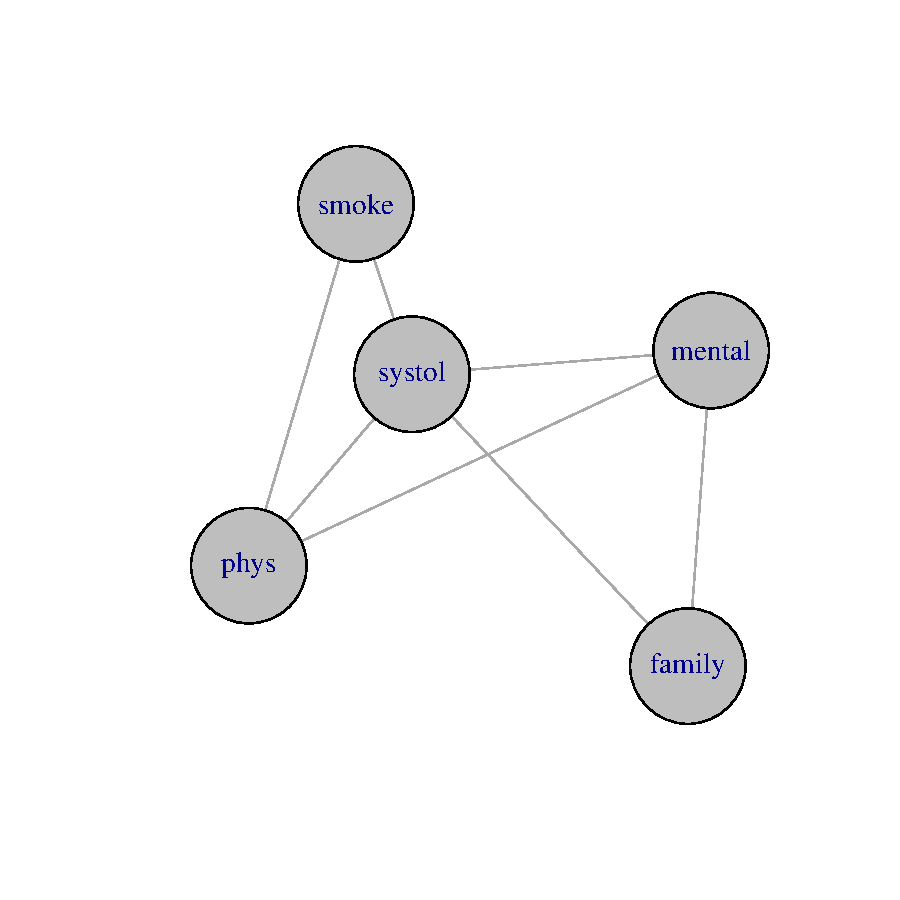
\includegraphics[]{figures/GRIM-fundamentalfig1}
  \caption{A decomposable graphical model for the \reinis\ data.}
  \label{fig:fundamentalfig1}
\end{figure}


\subsection{Testing for addition and deletion of edges}
\label{sec:xxx}

Let $\calM_0$ be a model and let $e=\{u,v\}$ be an edge in $\calM_0$.
The candidate model  formed by deleting $e$ from $\calM_0$ is $\calM_1$.
The \code{testdelete()} function can be used to test for deletion of
an edge from a model:

\begin{Schunk}
\begin{Sinput}
> testdelete(dm5, ~smoke:systol)
\end{Sinput}
\begin{Soutput}
dev:   11.698 df:  2 p.value: 0.00288 AIC(k=2.0):    7.7 edge: smoke:systol 
host:  systol phys smoke 
Notice: Test performed in saturated marginal model
\end{Soutput}
\begin{Sinput}
> testdelete(dm5, ~family:systol)
\end{Sinput}
\begin{Soutput}
dev:    1.085 df:  2 p.value: 0.58135 AIC(k=2.0):   -2.9 edge: family:systol 
host:  systol family mental 
Notice: Test performed in saturated marginal model
\end{Soutput}
\end{Schunk}


In the first case the $p$--value suggests that the edge can not be
deleted. In the second case the $p$--value suggests that the edge can
be deleted. The reported AIC
value is the difference in AIC between the candidate model and the
original model. A negative value of AIC suggest that the candidate
model is to be preferred.


Next, let $\calM_0$ be a model and let $e=\{u,v\}$ be an edge not in
$\calM_0$. The candidate model  formed by adding $e$ to $\calM_0$ is
denoted $\calM_1$.
The \code{testadd()} function can be used to test for deletion of
an edge from a model:

\begin{Schunk}
\begin{Sinput}
> testadd(dm5, ~smoke:mental)
\end{Sinput}
\begin{Soutput}
dev:    7.797 df:  4 p.value: 0.09930 AIC(k=2.0):   -0.2 edge: smoke:mental 
host:  mental systol phys smoke 
Notice: Test performed in saturated marginal model
\end{Soutput}
\end{Schunk}

The $p$--value suggests that no significant improvedment of the model
is obtained by adding the edge. The reported AIC value is the
difference in AIC between the candidate model and the original
model. A negative value of AIC would have suggested that the candidate
model is to be preferred.

\footnote{A function for testing addition / deletion of more general
  terms is needed.}



\subsection{Finding edges}
\label{sec:xxx}

The \code{getInEdges()} function will return a list of all the edges
in the dependency graph $\calG$ defined by the model. If we set
\code{type='decomposable'} then the edges returned are as follows: An
edge $e=\{u,v\}$ is returned if $\calG$ minus the edge $e$ is
decomposable. In connection with model selection this is convenient
because it is thereby possibly to restrict the search to decomposable
models.

\begin{Schunk}
\begin{Sinput}
> ed.in <- getInEdges(ugList(terms(dm5)), type="decomposable")
\end{Sinput}
\begin{Soutput}
     [,1]     [,2]    
[1,] "mental" "phys"  
[2,] "mental" "family"
[3,] "phys"   "smoke" 
[4,] "systol" "family"
[5,] "systol" "smoke" 
\end{Soutput}
\end{Schunk}

The \code{getOutEdges()} function will return a list of all the edges
which are not in the dependency graph $\calG$ defined by the model. If we set
\code{type='decomposable'} then the edges returned are as follows: An
edge $e=\{u,v\}$ is returned if $\calG$ plus the edge $e$ is
decomposable. In connection with model selection this is convenient
because it is thereby possibly to restrict the search to decomposable
models.


\begin{Schunk}
\begin{Sinput}
> ed.out <- getOutEdges(ugList(terms(dm5)), type="decomposable")
\end{Sinput}
\begin{Soutput}
     [,1]     [,2]    
[1,] "mental" "smoke" 
[2,] "phys"   "family"
\end{Soutput}
\end{Schunk}


\subsection{Testing several edges}
\label{sec:labeledges}

\begin{Schunk}
\begin{Sinput}
> args(testInEdges)
\end{Sinput}
\begin{Soutput}
function (object, edgeMAT = NULL, criterion = "aic", k = 2, alpha = NULL, 
    headlong = FALSE, details = 1, ...) 
NULL
\end{Soutput}
\begin{Sinput}
> args(testOutEdges)
\end{Sinput}
\begin{Soutput}
function (object, edgeMAT = NULL, criterion = "aic", k = 2, alpha = NULL, 
    headlong = FALSE, details = 1, ...) 
NULL
\end{Soutput}
\end{Schunk}



The functions \code{labelInEdges()} and \code{labelOutEdges()} will
test for deletion of edges and addition of edges. The default is to
use AIC for evaluating each edge. It is possible to specify the penalty parameter for AIC to being other
values than 2 and it is possible to base the evaluation on
significance tests instead of AIC. Setting \code{headlong=TRUE} causes
the function to exit once an improvement is found.
For example:

\begin{Schunk}
\begin{Sinput}
> testInEdges(dm5, getInEdges(ugList(terms(dm5)), type="decomposable"),
+              k=log(sum(reinis)))
\end{Sinput}
\begin{Soutput}
  statistic df   p.value     aic     V1     V2 action
1   686.703  2 0.000e+00 671.667 mental   phys      -
2     4.693  2 9.572e-02 -10.344 mental family      +
3    28.147  2 7.726e-07  13.111   phys  smoke      -
4     1.085  2 5.813e-01 -13.951 systol family      +
5    11.698  2 2.882e-03  -3.338 systol  smoke      +
\end{Soutput}
\end{Schunk}






\section{Stepwise model selection}
\label{sec:stepwise}

Two functions are currently available for model selection:
\code{backward()} and \code{forward()}. These functions employ the
functions in Section~\ref{sec:labeledges})


\subsection{Backward search}
\label{sec:xxx}

For example, we start with the saturated model and do a backward search.

\begin{Schunk}
\begin{Sinput}
> dm.sat <- dmod(~.^., data=reinis)
> dm.back <- backward(dm.sat)
\end{Sinput}
\begin{Soutput}
  change.AIC  -19.7744 Edge deleted: mental,systol
  change.AIC   -8.8511 Edge deleted: phys,systol
  change.AIC   -4.6363 Edge deleted: mental,protein
  change.AIC   -1.6324 Edge deleted: systol,family
  change.AIC   -3.4233 Edge deleted: family,protein
  change.AIC   -0.9819 Edge deleted: phys,family
  change.AIC   -1.3419 Edge deleted: smoke,family
\end{Soutput}
\begin{Sinput}
> iplot(dm.back)
\end{Sinput}
\end{Schunk}
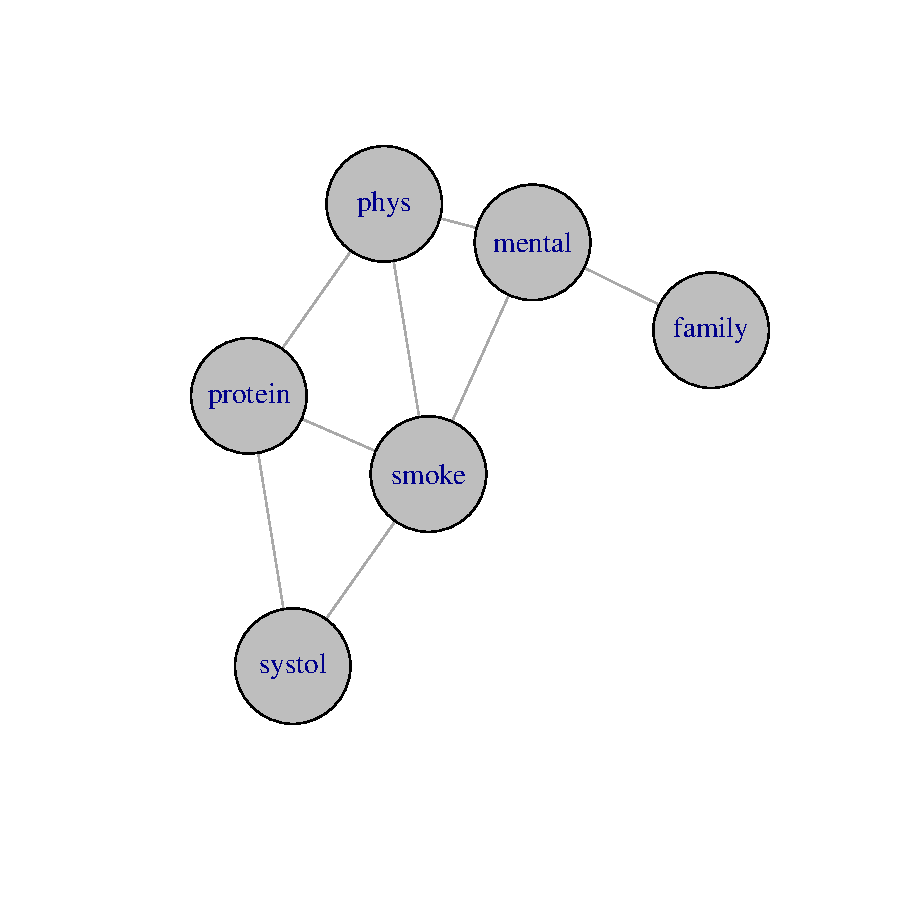
\includegraphics{figures/GRIM-034}

Default is to search among decomposable models if the initial model is
decomposable. Default is also to label all edges (with AIC values);
however setting \code{search='headlong'} will cause the labelling to
stop once an improvement has been found.

\subsection{Forward search}
\label{sec:xxx}

Forward search works similarly; for example we start from the
independence model:

\begin{Schunk}
\begin{Sinput}
> dm.i   <- dmod(~.^1, data=reinis)
> dm.forw <- forward(dm.i)
\end{Sinput}
\begin{Soutput}
  change.AIC   -1.9046 Edge added: phys,systol
  change.AIC   -1.8298 Edge added: phys,family
  change.AIC   -1.4999 Edge added: systol,mental
  change.AIC   -0.9313 Edge added: family,smoke
\end{Soutput}
\begin{Sinput}
> iplot(dm.forw)
\end{Sinput}
\end{Schunk}
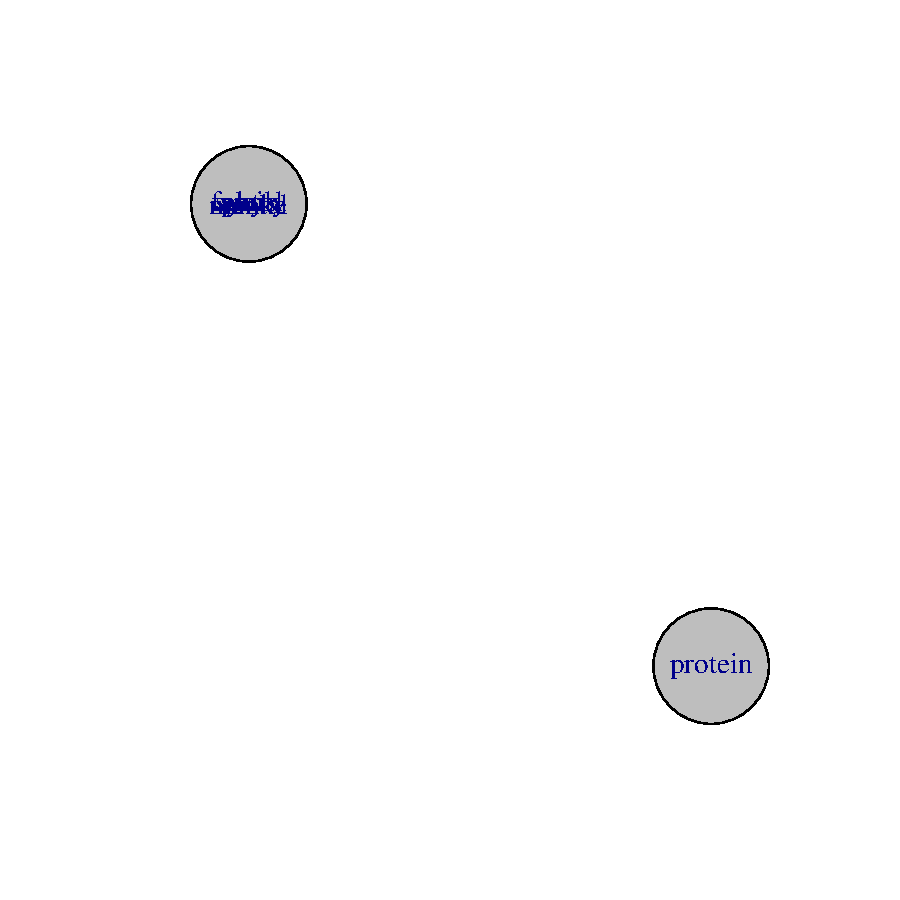
\includegraphics{figures/GRIM-035}

% \subsection{Backward and forward search}
% \label{sec:xxx}

% The \code{stepwise()} function will perform a stepwise model
% selection. Start from the saturated model:

% @
% <<>>=
% dm.s2<-stepwise(dm.sat, details=1)
% @ %def

% The default selection criterion is AIC (as opposed to significance
% test); the default penalty parameter in AIC is $2$ (which gives
% genuine AIC). The default search direction is backward (as opposed to
% forward). Default is to restrict the search to decomposable models if
% the starting model is decomposable; as opposed to unrestricted
% search. Default is not to do headlong search which means that all
% edges are tested and the best edge is chosen to delete. Headlong on
% the other hand means that once a deletable edge is encountered, then
% this edge is deleted.


% Likewise, we may do a forward search starting from the independence model:

% @
% <<>>=
% dm.i2<-stepwise(dm.i, direction="forward", details=1)
% @ %def


% @
% <<stepwise01, fig=T, include=F>>=
% par(mfrow=c(1,2))
% dm.s2
% dm.i2
% plot(dm.s2)
% plot(dm.i2)
% @ %def

% \begin{figure}[h]
%   \centering
%   \includegraphics{figures/GRIM-stepwise01}
%   \caption{Models for the \reinis\ data obtained by backward (left) and forward (right) stepwise model selection.}
%   \label{fig:stepwise01}
% \end{figure}


% Stepwise model selection is in practice only feasible for moderately sized
% problems.




\subsection{Fixing edges/terms in model as part of model selection}
\label{sec:xxx}

The stepwise model selection can be controlled by fixing specific
edges. For example we can specify edges which are not to be considered
in a bacward selection:

\begin{Schunk}
\begin{Sinput}
> fix <- list(c("smoke","phys","systol"), c("systol","protein"))
> fix <- do.call(rbind, unlist(lapply(fix, names2pairs),recursive=FALSE))
> fix
\end{Sinput}
\begin{Soutput}
     [,1]      [,2]    
[1,] "phys"    "smoke" 
[2,] "smoke"   "systol"
[3,] "phys"    "systol"
[4,] "protein" "systol"
\end{Soutput}
\begin{Sinput}
> dm.s3 <- backward(dm.sat, fixin=fix, details=1)
\end{Sinput}
\begin{Soutput}
  change.AIC  -19.7744 Edge deleted: mental,systol
  change.AIC   -4.6982 Edge deleted: systol,family
  change.AIC   -6.8301 Edge deleted: protein,family
  change.AIC   -1.2294 Edge deleted: mental,protein
  change.AIC   -0.9819 Edge deleted: phys,family
  change.AIC   -1.3419 Edge deleted: smoke,family
\end{Soutput}
\end{Schunk}

There is an important detail here: The matrix \code{fix} specifies a
set of edges. Submitting these in a call to \comic{backward} does
not mean that these edges are forced to be in the model. It means that
those edges in \code{fixin} which are in the model will not be removed.

Likewise in forward selection:

\begin{Schunk}
\begin{Sinput}
> dm.i3 <- forward(dm.i, fixout=fix, details=1)
\end{Sinput}
\begin{Soutput}
  change.AIC   -1.8298 Edge added: phys,family
  change.AIC   -1.4999 Edge added: mental,systol
  change.AIC   -0.9313 Edge added: smoke,family
  change.AIC   -0.8762 Edge added: systol,family
\end{Soutput}
\end{Schunk}

Edges in \code{fix} will not be added to the model but if they are in
the starting model already, they will remain in the final model.


% @
% <<stepwise02, fig=T, include=F>>=
% par(mfrow=c(1,2))
% dm.s3
% dm.i3
% plot(dm.s3)
% plot(dm.i3)
% @ %def

% \begin{figure}[h]
%   \centering
%   \includegraphics{figures/GRIM-stepwise02}
%   \caption{Models for the \reinis\ data obtained by backward (left)
%     and forward (right) stepwise model selection when certain edges
%     are restricted in the selection procedure. }
%   \label{fig:stepwise02}
% \end{figure}




\section{Further topics on models for contingency tables}
\label{sec:xxx}


\subsection{Adjusting for sparsity}
\label{sec:xxx}

\footnote{Comment on adjustment for sparsity in testadd() and testdelete()}


% \subsection{Sparse Contingency Tables}
% \label{sec:xxx}



% @
% <<fig=T>>=
%  data(mildew)
%  dm1 <- dmod(~.^., data=mildew)
%  dm1
%  dm2 <- stepwise(dm1)
%  dm2
%  plot(dm2)
% @ %def



% \subsection{A space--efficient implementation of IPS for contingency tables}
% \label{sec:xxx}

% \footnote{effloglin() is not the best name. Perhaps loglineff() is a bit
%   better. Should start with loglin...}

% Consider a hierarchical log--linear model with generating class $\calA
% = \{a_1, \dots, a_M\}$ over a set of variables $\Delta$.  The
% Iterative Proportional Scaling (IPS) algorithm (as described e.g.\ in
% \cite{lauritzen:96}, p.\ 83) as a commonly used method for fitting
% such models. The updating steps are of the form
% \begin{displaymath}
%   p(i) \leftarrow p(i)\frac{n(i_{a_k})/n}{p(i_{a_k})} \mbox{ for } k=1,\dots,M.
% \end{displaymath}

% The IPS algorithm is implemented in the \comic{loglin()} function.
% The IPS algorithm is \emph{inefficient} in the sense that it requires
% the entire table to be fitted. For example, if there are $81$ variables
% each with $10$ levels then a table with $10^{81}$ will need to be created.
% (Incidently, $10^{81}$ is one of the figures reported as the number of
% atoms in the universe. It is a large number!).

% A more \emph{efficient} IPS algorithm is described by
% \cite{jirousek:preucil:95}, and this is implemented in the
% \comic{effloglin()} function. The implementation of
% \comi{effloglin()} is made entirely in \R\ and therefore the word
% \emph{efficient} should be understood in terms of space
% requirement (for small problems, \comi{loglin()} is much faster than
% \comi{effloglin()}).

% The algorithm goes as follows: It is assumed that $\calA$ is minimally
% specified, i.e.\ that no element in $\calA$ is contained in another
% element in $\calA$.  Form the dependency graph $\calG(\calA)$ induced by
% $\calA$. Let $\calG'$ denoted a triangulation of $\calG(\calA)$ and  let
% $\calC=\{C_1,\dots,C_N\}$ denote the cliques of $\calG'$.
% Each $a\in \calA$ is then contained in exactly one clique $C\in
% \calC$. Let $\calA_C=\{a\in \calA:a\subset C\}$ so that $\calA_{C_1},
% \dots, \calA_{C_N}$ is a disjoint partitioning of $\calA$.

% Any probability $p$ satisfying the constraints of $\calA$ will also factorize
% according to $\calG'$ so that
% \begin{equation}
%   \label{eq:effloglin1}
%   p(i) = \prod_{C\in \calC} \psi_C(i_C)
% \end{equation}


% Using e.g.\ the computation architecture of
% \cite{lauritzen:spiegelhalter:88} the clique marginals
% \begin{equation}
%   \label{eq:effloglin2}
%   p_{C}(i_{C}), \quad C \in \calC
% \end{equation}
% can be obtained from (\ref{eq:effloglin1}). In practice calculation of
% (\ref{eq:effloglin2}) is done using the \grain\ package.
% For $C\in \calC$ and an $a \in \calA_C$ update $\psi_C$ in
% (\ref{eq:effloglin1}) as
% \begin{displaymath}
%   \psi_C(i_C) \leftarrow \psi_C(i_C) \frac{n(i_a)/n}{p_a(i_a)}
% \end{displaymath}
% where $p_a$ is obtained by summing over variables in $C\setminus
% a$ in $p_C$ from (\ref{eq:effloglin2}). Then find the new clique
% marginals in (\ref{eq:effloglin2}), move on to the next $a$ in
% $\calA_{C}$ and so on.




% As an example, consider 4--cycle model for reinis data:

% @
% <<>>=
% data(reinis)
% ff    <- ~smoke:mental+mental:phys+phys:systol+systol:smoke
% dmod(ff, data=reinis)
% @ %def


% This model can be fitted with \code{loglin()} as

% @
% <<>>=
% glist <- rhsFormula2list(ff)
% glist
% fv1 <- loglin(reinis, glist, print=FALSE)
% fv1[1:3]
% @ %def

% An alternative is \code{effloglin()} which uses the algorithm above
% triangulated graph:

% @
% <<>>=
% fv2 <- effloglin(reinis, glist, print=FALSE)
% fv2[c('logL','nparm','df')]
% @ %def

% The real virtue of \code{effloglin()} lies in that it is possible to
% submit data as a list of sufficient marginals:

% @
% <<>>=
% stab <- lapply(glist, function(gg) tableMargin(reinis, gg))
% fv3 <- effloglin(stab, glist, print=FALSE)
% @ %def

% A sanity check:

% @
% <<>>=
% f1 <- loglin(reinis, glist, print=F, fit=T)$fit
% f3 <- effloglin(stab, glist, print=F, fit=T)$fit
% f1 <- tableMargin(f1, names(dimnames(f3)))
% max(abs(f1-f3))
% @ %def

% Notice the timings

% @
% <<>>=
% system.time({ for (ii in 1:100) loglin(reinis, glist, print=FALSE)})
% system.time({ for (ii in 1:100) effloglin(stab, glist, print=FALSE)})
% @ %def


% @
% <<>>=
% system.time({ for (ii in 1:100) loglin(reinis, glist, fit=FALSE, print=FALSE)})
% system.time({ for (ii in 1:100) effloglin(stab, glist, fit=FALSE, print=FALSE)})
% @ %def




% @
% <<>>=
% Rprof()
% system.time({ for (ii in 1:100) effloglin(stab, glist, print=FALSE)})
% Rprof(NULL)
% summaryRprof()
% @ %def


\subsection{Dimension of a log--linear model}
\label{sec:dimloglin}

The \code{loglinDim()} is a general function for finding the dimension
of a log--linear model. It works on the generating class of a model
being represented as a list:

\begin{Schunk}
\begin{Sinput}
> dim_loglin(terms(dm2), reinis)
\end{Sinput}
\begin{Soutput}
[1] 10
\end{Soutput}
\end{Schunk}

% Consider the model for the \code{mildew} data given by the formula
% (see Figure~\ref{fig:dimension})

% @
% <<>>=
% ff <- ~la10:locc:mp58:c365+mp58:c365:p53a:a367
% @ %def

% <<dimension,fig=T,include=F,echo=F>>=
% plot(ug(ff))
% @ %def

% \begin{figure}[h]
%   \centering
%   \includegraphics[height=5cm]{figures/GRIM-dimension}
%   \caption{A decomposable graphical model for the \code{mildew} data.}
%   \label{fig:dimension}
% \end{figure}


% As the model defined above is decomposable it is possible to calculate
% and adjusted dimension which accounts for sparsity of data with \code{loglinDecDim()}:

% @
% <<>>=
% loglinDecDim(glist, mildew)
% @ %def

% These adjusments are accounted for when creating log--linear models:

% @
% <<>>=
% dmod(ff, data=mildew)
% @ %def



\section{Miscellaneous}
\label{sec:misc}





\subsection{The Model Object}
\label{sec:intomodel}


It is worth looking at the information in the model object:

\begin{Schunk}
\begin{Sinput}
> dm3 <- dmod(list(c("smoke", "systol"), c("smoke", "mental", "phys")),
+             data=reinis)
> names(dm3)
\end{Sinput}
\begin{Soutput}
[1] "modelinfo" "varNames"  "datainfo"  "fitinfo"   "isFitted" 
\end{Soutput}
\end{Schunk}

\begin{itemize}

\item The model, represented as a list of generators, is

\begin{Schunk}
\begin{Sinput}
> str(terms(dm3))
\end{Sinput}
\begin{Soutput}
List of 2
 $ : chr [1:3] "smoke" "mental" "phys"
 $ : chr [1:2] "smoke" "systol"
\end{Soutput}
\end{Schunk}

\begin{Schunk}
\begin{Sinput}
> str(dm3$glistNUM)
\end{Sinput}
\begin{Soutput}
 NULL
\end{Soutput}
\end{Schunk}

The numeric representation of the generators refers back to

\begin{Schunk}
\begin{Sinput}
> dm3$varNames
\end{Sinput}
\begin{Soutput}
[1] "smoke"  "mental" "phys"   "systol"
\end{Soutput}
\end{Schunk}

Notice the model object does not contain a graph object. Graph objects
are generated on the fly when needed.

\item Information about the variables etc. is

\begin{Schunk}
\begin{Sinput}
> str(dm3[c("varNames","conNames","conLevels")])
\end{Sinput}
\begin{Soutput}
List of 3
 $ varNames: chr [1:4] "smoke" "mental" "phys" "systol"
 $ NA      : NULL
 $ NA      : NULL
\end{Soutput}
\end{Schunk}

\item Finally \code{isFitted} is a logical for whether the model is fitted;
  \code{data} is the data (as a table) and \code{fitinfo} consists of
  fitted values, logL, df etc.
\end{itemize}



%%\listoffixmes


\end{document}



% \section{Testing for addition and deletion of edges}
% \label{sec:xxx}

% Consider the saturated and the independence models for the
% \code{carcass} data:

% @
% <<print=T>>=
% data(carcass)
% cm1 <- cmod(~.^., carcass)
% cm2 <- cmod(~.^1, data=carcass)
% @ %def


% \subsection{\code{testdelete()}}
% \label{sec:xxx}



% Let $\calM_0$ be a model and let $e=\{u,v\}$ be an edge in $\calM_0$.
% The candidate model  formed by deleting $e$ from $\calM_0$ is $\calM_1$.
% The \code{testdelete()} function can be used to test for deletion of
% an edge from a model:

% @
% <<>>=
% testdelete(cm1,~M11:F11)
% testdelete(cm1,~M12:F13)
% @ %def

% In the first case the $p$--value suggests that the edge can not be
% deleted. In the second case the $p$--value suggests that the edge can
% be deleted. The reported AIC
% value is the difference in AIC between the candidate model and the
% original model. A negative value of AIC suggest that the candidate
% model is to be preferred.


% \subsection{\code{testadd()}}
% \label{sec:xxx}

% Next, let $\calM_0$ be a model and let $e=\{u,v\}$ be an edge not in
% $\calM_0$. The candidate model  formed by adding $e$ to $\calM_0$ is
% denoted $\calM_1$.
% The \code{testadd()} function can be used to test for deletion of
% an edge from a model:

% @
% <<>>=
% testadd(cm2, ~M11:F11)
% testadd(cm2, ~M12:F13)
% @ %def


% In the first case the $p$--value suggests that no significant
% improvedment of the model is obtained by adding the edge. In the
% second case a significant improvement is optained by adding the edge.
% The reported AIC
% value is the difference in AIC between the candidate model and the
% original model. A negative value of AIC suggest that the candidate
% model is to be preferred.


% \section{Finding edges}
% \label{sec:xxx}

% Consider the following model for the \carcass\ data:

% @
% <<fig=T>>=
% data(carcass)
% cm1 <- cmod(~LMP:M12:F12+LMP:F11:F12+F11:F12:F13, data=carcass)
% plot(cm1)
% @ %def

% \subsection{\code{getInEdges()}}
% \label{sec:xxx}


% The edges in the model are

% @
% <<>>=
% getInEdges(cm1)
% @ %def

% In connection with model selection it is sometimes convenient to get
% only the edges which are contained in only one clique:

% @
% <<>>=
% getInEdges(cm1, type="decomposable")
% @ %def

% \footnote{getInEdges/getOutEdges: type=''decomposable'' is a silly value for the argument}

% \footnote{getInEdges/getOutEdges: Should be possible to have edges as a
%   matrix instead. Perhaps even as default.}

% \subsection{\code{getOutEdges()}}
% \label{sec:xxx}

% The edges not in the model are

% @
% <<>>=
% getOutEdges(cm1)
% @ %def

% In connection with model selection it is sometimes convenient to get
% only the edges which when added will be in only one clique of the new model:

% @
% <<>>=
% getOutEdges(cm1, type="decomposable")
% @ %def


% \section{Evaluating edges in the model}
% \label{sec:xxx}

% @
% <<fig=T>>=
% data(carcass)
% cm1 <- cmod(~LMP:M12:F12+LMP:F11:F12+F11:F12:F13+F12:M11:M13, data=carcass[1:20,])
% plot(cm1)
% @ %def

% \subsection{\code{evalInEdges()}}
% \label{sec:xxx}

% @
% <<>>=
% in.ed <- getInEdges(cm1)
% z<-evalInEdges(cm1, edgeList=in.ed)
% @ %def

% Hence there are four edges which lead to a decrease in AIC. If we set
% \code{headlong=T} then the function exist as soon as one decrease in
% AIC is found:

% @
% <<>>=
% z<-evalInEdges(cm1, edgeList=in.ed, headlong=T)
% @ %def


% \subsection{\code{evalOutEdges()}}
% \label{sec:xxx}

% @
% <<>>=
% out.ed <- getOutEdges(cm1)
% z<-evalOutEdges(cm1, edgeList=out.ed)
% @ %def

% Hence there are four edges which lead to a decrease in AIC. If we set
% \code{headlong=T} then the function exist as soon as one decrease in
% AIC is found:

% @
% <<>>=
% z<-evalOutEdges(cm1, edgeList=out.ed, headlong=T)
% @ %def


% \section{Methods for model objects}
% \label{sec:ccc}



% A \comi{summary()} of a model:

% @
% <<>>=
% summary(dm1)
% @ %def



% @
% <<>>=
% str(fitted(dm1))
% str(dm1$data)
% @ %def

% Hence we can make a simple diagnostic plot of Pearson residuals as

% @
% <<pearson-1,fig=T,include=F>>=
% X2 <- (fitted(dm1)-dm1$datainfo$data)/sqrt(fitted(dm1))
% qqnorm(as.numeric(X2))
% @ %def

% \begin{figure}[h]
%   \centering
%   \includegraphics[]{figures/GRIM-pearson-1}
%   \caption{A marginal model for a slice of the \reinis\ data.}
%   \label{fig:pearson-1}
% \end{figure}




% @
% <<>>=
% str(dm1$glist)
% @ %def
